\documentclass[11pt,a4paper]{paper}

\usepackage{preambule}
\fancyhead[L]{\scriptsize \textsc{Nora Nicolas}}

\begin{document}

\title{Referee answer}

\section{Of the surveys' spectroscopic follow-up}
\begin{enumerate}

    \item SNLS's detection efficiency $\e \approx 0$ for $i \approx
        \SI{24.8}{mag}$\smallbreak

        \textcolor{red}{A limiting magnitude of $m_{\lim} = \SI{23.5}{mag}
        \Rightarrow z_{\lim} = 0.36$, which would lead to only 26/236 SNe
    instead of 102/236 with our current cut}
    
    \item HST may have a follow-up efficiency that we should take into account
        like we did for SDSS;

    \item Misunderstanding about the 20\% of SNf's SNe that had selection
        effects:\smallbreak

        \textcolor{dgreen}{The 80\% of SNf's SNe that had no selection
effects are the 114 SNe that are in our sample}.
\end{enumerate}

\section{Of the $x_1$ bias that doesn't appear on $m$}
The referee insists on the fact that ``Biases in x1 are expected as a function
of redshift simply from survey modeling/selection effects'', showing the
following figure from \textsc{Kessler \& Scolnic 2017} to point
out that biases in $x_1$ become apparent much sooner that biases on $m$.

\begin{figure}[htbp!]
    \centering
    \begin{subfigure}
        \centering
        \includegraphics[width=.3\linewidth]{Answer_figures/Fig_biasCor_mb.eps}
    \end{subfigure}
    \begin{subfigure}
        \centering
        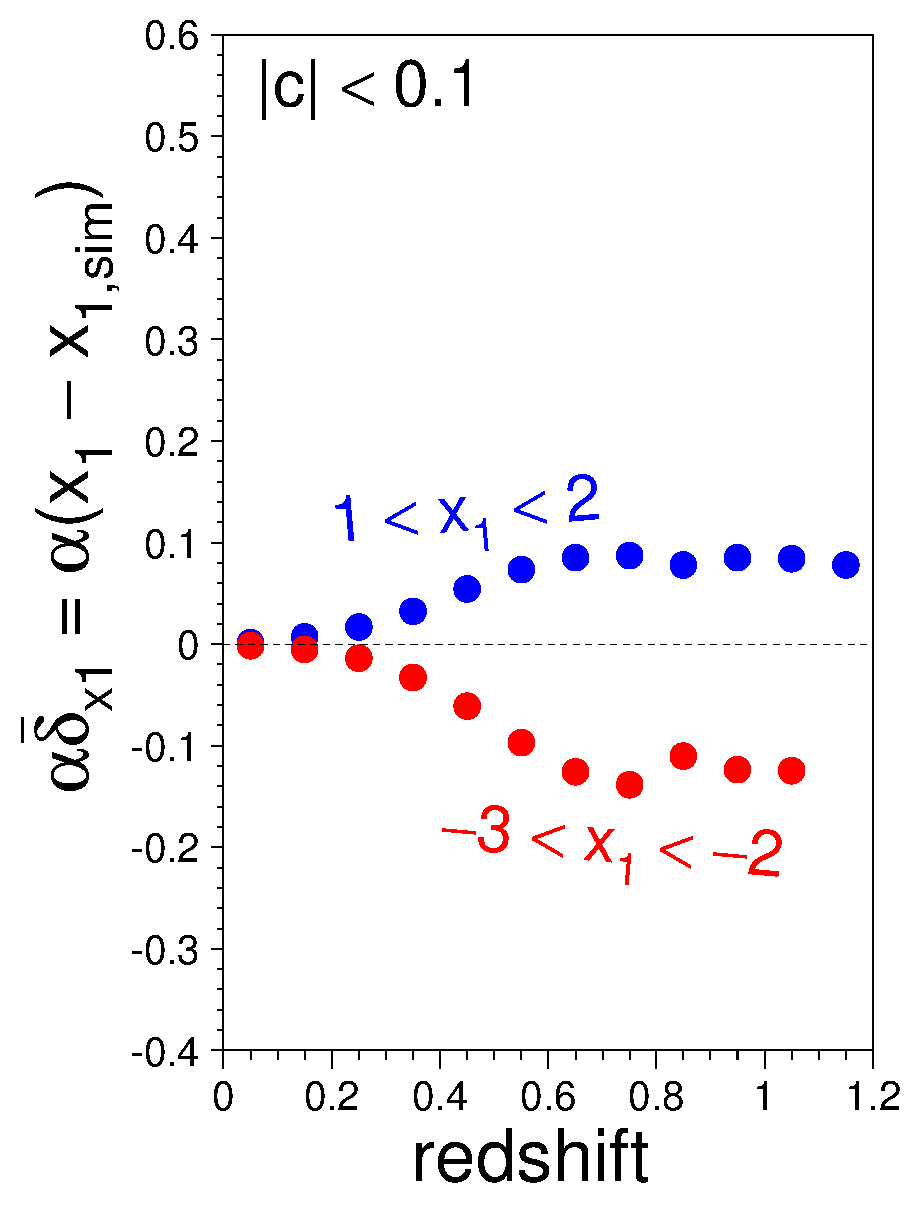
\includegraphics[width=.3\linewidth]{Answer_figures/Fig_biasCor_x1.eps}
    \end{subfigure}
    \begin{subfigure}
        \centering
        \includegraphics[width=.3\linewidth]{Answer_figures/Fig_biasCor_c.eps}
    \end{subfigure}
    \captionsetup{justification=centering}
    \caption{Bias corrections $\mkern
        1.5mu\overline{\mkern-1.5mu\delta\mkern-1.5mu}\mkern 1.5mu_{m_B}$,
        $\alpha \overline{\delta}_{x_1}$, and $\beta\overline{\delta}_{c}$ are
        shown as a function of redshift. The pre-factors $\alpha, \beta$ are
        used to show the bias in distance-modulus magnitudes. The parameter
    selection ranges are shown on each panel.}
    \label{fig:KS17}
\end{figure}

\begin{wrapfigure}[10]{R}{.4\linewidth}
    \vspace*{-20pt}
    \centering
    \includegraphics[width=\linewidth]{Answer_figures/hist_surveys2_btw_cividis.pdf}
    \captionsetup{justification=centering}
    \caption{\small Redshift histograms of SNe~Ia from the SDSS and PS1 datasets
    respectively}
    \label{fig:hists}
\end{wrapfigure}
Yet, from the same figure, biases in $c$ appear at $z=0$. Here we want to
convince the referee that if we don't find any sign of color bias in our sample,
we may consider little to no bias on $x_1$. We thus studied the $x_1$ and $c$
distributions of the end of SDSS and the start of PS1, for $0.10 < z < 0.20$. In
this redshift range, the SDSS cut dataset contains the most questionable SNe~Ia,
for the SNe between $0.15 < z < 0.20$ are between our conservative and fiducial
cuts, due to limited spectroscopic resources; the PS1 dataset is however quite
robust for these SNe are far from both the conservative and fiducial cuts; see
Fig. \ref{fig:hists}. \bigbreak

The results are shown Fig. \ref{fig:distrib}

\begin{figure}[htbp!]
    \centering
    \includegraphics[width=\linewidth]{Answer_figures/both-cut_SDSS_PS1-010-020.pdf}
    \captionsetup{justification=centering}
    \caption{$x_1$ and $c$ distributions of the SDSS and PS1 samples for $0.10 <
    z < 0.20$. A Kolmogorov-Smirnov test doesn't show any indication that the
samples are not taken from the same distribution.}
\label{fig:distrib}
\end{figure}

\end{document}
